\documentclass{amsart}
\usepackage{a4wide}
\usepackage{tikz,pgfmath}

\definecolor{olivegreen}{cmyk}{0.64,0,0.95,0.40}

\begin{document}


% 3.1.3
\begin{center}
 \begin{tikzpicture}[scale=1.5] % [30]{-2.2}{2.2}{-2.2}{2.2}
  \draw[->] (-2.2,0) -- (2.2,0);
  \draw[->] (0,-2.2) -- (0,2.2);
  \draw[dotted] (-2,-2) -- (-2,+2);
  \draw[dotted] (-1,-2) -- (-1,+2);
  \draw[dotted] ( 1,-2) -- ( 1,+2);
  \draw[dotted] ( 2,-2) -- ( 2,+2);
  \draw[dotted] (-2,-2) -- (+2,-2);
  \draw[dotted] (-2,-1) -- (+2,-1);
  \draw[dotted] (-2, 1) -- (+2, 1);
  \draw[dotted] (-2, 2) -- (+2, 2);
  \draw[dotted] (0,0) circle(1);

  \fill[red] ( 1, 0) circle(0.04);
  \fill[red] (-1, 0) circle(0.04);
  \fill[red] ( 0, 1) circle(0.04);
  \fill[red] ( 0,-1) circle(0.04);

  \draw ( 1.1, 0.1) node[anchor=south west] {$\scriptstyle ( 1, 0)$};
  \draw (-0.1, 1.1) node[anchor=south east] {$\scriptstyle ( 0, 1)$};
  \draw (-1.1,-0.1) node[anchor=north east] {$\scriptstyle (-1, 0)$};
  \draw ( 0.1,-1.1) node[anchor=north west] {$\scriptstyle ( 0,-1)$};
 \end{tikzpicture}
\end{center}


% 3.2.3
\begin{center}
 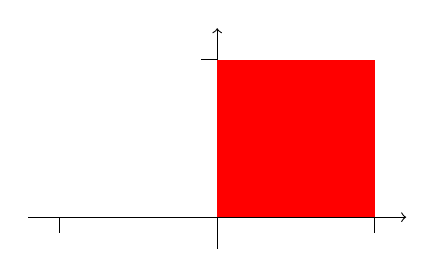
\begin{tikzpicture}[scale=2]
  \draw[->] (-1.2,0) -- (1.2,0);
  \draw[->] (0,-0.2) -- (0,1.2);
  \draw (-1,0) -- (-1,-0.1);
  \draw ( 0,0) -- ( 0,-0.1);
  \draw (+1,0) -- (+1,-0.1);
  \draw (-0.1,1) -- (0,1);
  \fill[red] (0,0) rectangle(1,1);
 \end{tikzpicture}
\end{center}

% 3.2.3
\begin{center}
 \begin{tikzpicture}[scale=2]
  \draw[->] (-1.2,0) -- (1.2,0);
  \draw[->] (0,-1.2) -- (0,1.2);
  \foreach \x in {-1,0,1} \draw (\x,-0.1) -- (\x,0);
  \foreach \y in {-1,0,1} \draw (-0.1,\y) -- (0,\y);
  \draw[red] (0,0) circle(1);
  \fill ( 1, 0) circle(0.02);
  \fill ( 0, 1) circle(0.02);
  \fill (-1, 0) circle(0.02);
  \fill ( 0,-1) circle(0.02);
  \draw ( 1.1, 0.1) node[anchor=south west] {$( 1, 0)$};
  \draw (-0.1, 1.1) node[anchor=south east] {$( 0, 1)$};
  \draw (-1.1,-0.1) node[anchor=north east] {$(-1, 0)$};
  \draw ( 0.1,-1.1) node[anchor=north west] {$( 0,-1)$};
 \end{tikzpicture}
\end{center}

% 3.3.2
\begin{center}
 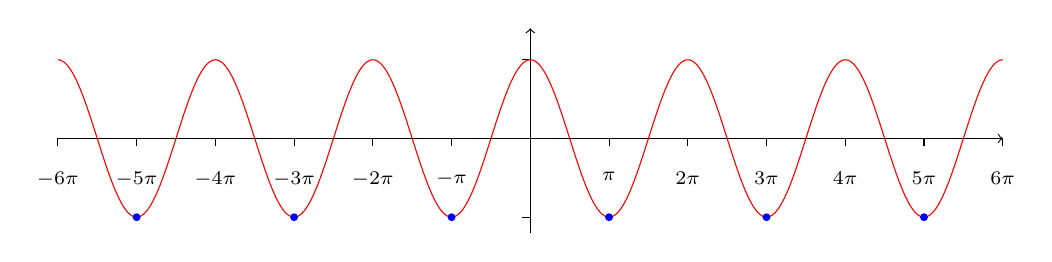
\begin{tikzpicture} % [25]{-6}{6}{-1.2}{1.4}
  \draw[->] (-6,0) -- (6,0);
  \draw[->] (0,-1.2) -- (0,1.4);
  \foreach \x in {-6 ,..., 6} \draw (\x,-0.1) -- (\x,0);
  \foreach \y in {-1 ,..., 1} \draw (-0.1,\y) -- (0,\y);
  \draw (-6,-.3) node[anchor=north] {$\scriptstyle -6\pi$};
  \draw (-5,-.3) node[anchor=north] {$\scriptstyle -5\pi$};
  \draw (-4,-.3) node[anchor=north] {$\scriptstyle -4\pi$};
  \draw (-3,-.3) node[anchor=north] {$\scriptstyle -3\pi$};
  \draw (-2,-.3) node[anchor=north] {$\scriptstyle -2\pi$};
  \draw (-1,-.3) node[anchor=north] {$\scriptstyle  -\pi$};
  \draw ( 1,-.3) node[anchor=north] {$\scriptstyle \pi$};
  \draw ( 2,-.3) node[anchor=north] {$\scriptstyle 2\pi$};
  \draw ( 3,-.3) node[anchor=north] {$\scriptstyle 3\pi$};
  \draw ( 4,-.3) node[anchor=north] {$\scriptstyle 4\pi$};
  \draw ( 5,-.3) node[anchor=north] {$\scriptstyle 5\pi$};
  \draw ( 6,-.3) node[anchor=north] {$\scriptstyle 6\pi$};
  \draw[red,domain=-6:6,samples=300,smooth,variable=\x]
    plot({\x},{cos(180*\x)});
  \begin{scope}[color=blue]
   \fill (-5,-1) circle(0.05);
   \fill (-3,-1) circle(0.05);
   \fill (-1,-1) circle(0.05);
   \fill ( 1,-1) circle(0.05);
   \fill ( 3,-1) circle(0.05);
   \fill ( 5,-1) circle(0.05);
  \end{scope}
 \end{tikzpicture}
\end{center}

% 3.4.3
{ \def\X{5.4}\def\A{0.75}\def\B{2.25}\def\C{3.15}\def\D{4.95}\def\Y{0}
\newcommand{\newset}[2]{%
 \def\Y{-#1}%
 \draw[black,dotted] (0,\Y/2) -- (\X,\Y/2);%
 \draw (6.3,\Y/2) node[anchor=west]{$#2$};%
}
\newcommand{\pp}[1]{\fill (#1,\Y/2) circle(0.05);}
\newcommand{\oo}[2]{\draw[ultra thick,red] (#1+0.09,\Y/2) -- (#2-0.09,\Y/2);}
\newcommand{\oc}[2]{\draw[ultra thick,red] (#1+0.09,\Y/2) -- (#2,\Y/2); \pp{#2}}
\newcommand{\co}[2]{\draw[ultra thick,red] (#1,\Y/2) -- (#2-0.09,\Y/2); \pp{#1}}
\newcommand{\cc}[2]{\draw[ultra thick,red] (#1,\Y/2) -- (#2,\Y/2); \pp{#1}\pp{#2}}
\begin{center}
 \begin{tikzpicture}
  \newset{0}{[a,b]} \cc{\A}{\B}
  \newset{1}{[b,c]} \cc{\B}{\C}
  \newset{2}{[a,b]\cup [b,c]=[a,c]} \cc{\A}{\C}
  \draw[white] (9,0) -- (10.5,0);
 \end{tikzpicture}
\end{center}
\begin{center}
 \begin{tikzpicture}
  \newset{0}{[a,d]} \cc{\A}{\D}
  \newset{1}{(b,c)} \oo{\B}{\C}
  \newset{2}{[a,d]\setminus(b,c)=[a,b]\cup [c,d]} \cc{\A}{\B} \cc{\C}{\D}
  \draw[white] (9,0) -- (10.5,0);
 \end{tikzpicture}
\end{center}
\begin{center}
 \begin{tikzpicture}
  \newset{0}{[a,c]} \cc{\A}{\C}
  \newset{1}{[b,d]} \cc{\B}{\D}
  \newset{2}{[a,c]\cap[b,d]=[b,c]} \cc{\B}{\C}
  \draw[white] (9,0) -- (10.5,0);
 \end{tikzpicture}
\end{center}
\begin{center}
 \begin{tikzpicture}
  \newset{0}{[a,c]} \cc{\A}{\C}
  \newset{1}{[b,d]} \cc{\B}{\D}
  \newset{2}{[a,c]\cap[b,d]=[b,c]} \cc{\B}{\C}
  \newset{3}{[a,c]\setminus [b,d]=[a,b)} \co{\A}{\B}
  \draw[white] (9,0) -- (10.5,0);
 \end{tikzpicture}
\end{center}
\begin{center}
 \begin{tikzpicture}
  \newset{0}{(a,d)} \oo{\A}{\D}
  \newset{1}{\{b,c\}} \pp{\B} \pp{\C}
  \newset{2}{(a,d)\setminus\{b,c\}} \oo{\A}{\B} \oo{\B}{\C} \oo{\C}{\D}
  \newset{3}{(a,b)} \oo{\A}{\B}
  \newset{4}{(b,c)} \oo{\B}{\C}
  \newset{5}{(c,d)} \oo{\C}{\D}
  \draw[white] (9,0) -- (10.5,0);
 \end{tikzpicture}
\end{center}
}

% 3.4.5
\begin{center}
 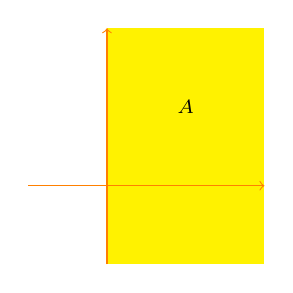
\begin{tikzpicture}
  \fill[yellow] (0,-1) -- (0,2) -- (2,2) -- (2,-1) -- cycle;
  \draw[orange,->] (-1,0) -- (2,0);
  \draw[orange,->] (0,-1) -- (0,2);
  \draw (1,1) node {$\scriptstyle A$};
 \end{tikzpicture}
 \hspace{2em}
 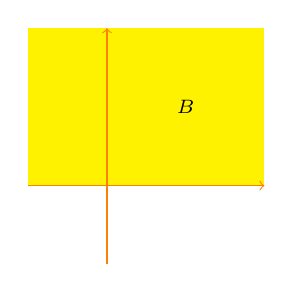
\begin{tikzpicture}
  \fill[yellow] (-1,0) -- (2,0) -- (2,2) -- (-1,2) -- cycle;
  \draw[orange,->] (-1,0) -- (2,0);
  \draw[orange,->] (0,-1) -- (0,2);
  \draw (1,1) node {$\scriptstyle B$};
 \end{tikzpicture}
 \hspace{2em}
 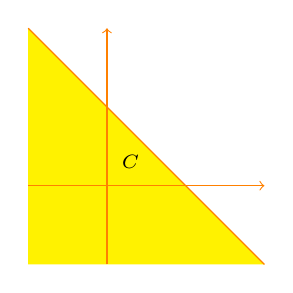
\begin{tikzpicture}
  \fill[yellow] (-1,-1) -- (-1,2) -- (2,-1) -- cycle;
  \draw[orange] (-1,2) -- (2,-1);
  \draw[orange,->] (-1,0) -- (2,0);
  \draw[orange,->] (0,-1) -- (0,2);
  \draw (.3,.3) node {$\scriptstyle C$};
 \end{tikzpicture}
 \hspace{2em}
 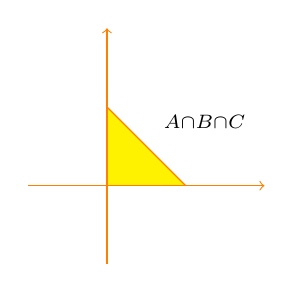
\begin{tikzpicture}
  \fill[yellow] (0,0) -- (0,1) -- (1,0) -- cycle;
  \draw[orange] (0,1) -- (1,0);
  \draw[orange,->] (-1,0) -- (2,0);
  \draw[orange,->] (0,-1) -- (0,2);
  \draw (.6,.6) node[anchor=south west] {$\scriptstyle A\cap B\cap C$};
 \end{tikzpicture}
\end{center}

% 3.4.8
\begin{center}
 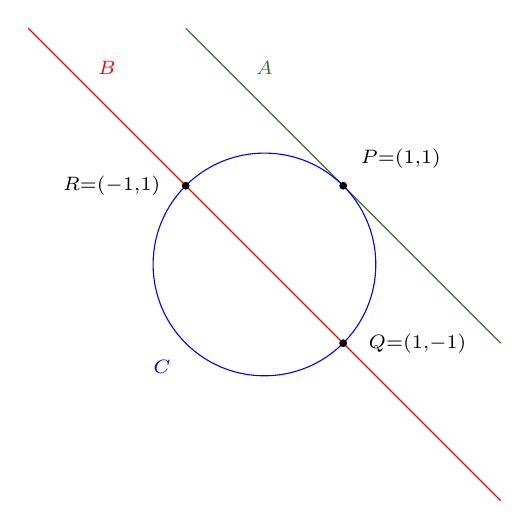
\begin{tikzpicture}
  \draw[olivegreen] (-1,3) -- (3,-1);
  \draw[olivegreen] (0,2.5) node {$\scriptstyle A$};
  \draw[red] (-3,3) -- (3,-3);
  \draw[red] (-2,2.5) node {$\scriptstyle B$};
  \draw[blue] (0,0) circle(1.4142135);
  \draw[blue] (-1.3,-1.3) node {$\scriptstyle C$};
  \fill ( 1, 1) circle(0.05);
  \fill (-1, 1) circle(0.05);
  \fill ( 1,-1) circle(0.05);
  \draw ( 1.1, 1.1) node[anchor=south west] {$\scriptstyle P=(1,1)$};
  \draw ( 1.2,-1.0) node[anchor=west] {$\scriptstyle Q=(1,-1)$};
  \draw (-1.2, 1.0) node[anchor=east] {$\scriptstyle R=(-1,1)$};
 \end{tikzpicture}
\end{center}

% 3.5.2
{ \def\X{4}\def\A{0.75}\def\B{2.25}\def\C{3.15}\def\D{4.95}\def\Y{0}
\newcommand{\newset}[2]{%
 \def\Y{-#1}%
 \draw[black,dotted] (0,\Y/2) -- (\X,\Y/2);%
 \draw (6.3,\Y/2) node[anchor=west]{$#2$};%
}
\newcommand{\pp}[1]{\fill (#1,\Y/2) circle(0.05);}
\newcommand{\oo}[2]{\draw[ultra thick,red] (#1+0.09,\Y/2) -- (#2-0.09,\Y/2);}
\newcommand{\oc}[2]{\draw[ultra thick,red] (#1+0.09,\Y/2) -- (#2,\Y/2); \pp{#2}}
\newcommand{\co}[2]{\draw[ultra thick,red] (#1,\Y/2) -- (#2-0.09,\Y/2); \pp{#1}}
\newcommand{\cc}[2]{\draw[ultra thick,red] (#1,\Y/2) -- (#2,\Y/2); \pp{#1}\pp{#2}}
\begin{center}
 \begin{tikzpicture} % [30][15]{0}{6}{-7}{0.5}
  \newset{0}{A} \cc{0}{2}
  \newset{1}{B} \cc{1}{3}
  \newset{2}{A^c} \oc{2}{4}
  \newset{3}{B^c} \co{0}{1} \oc{3}{4}
  \newset{4}{A\cup B} \cc{0}{3}
  \newset{5}{A\cap B} \cc{1}{2}
  \newset{6}{A^c\cup B^c=(A\cap B)^c} \co{0}{1} \oc{2}{4}
  \newset{7}{A^c\cap B^c=(A\cup B)^c} \oc{3}{4}
 \end{tikzpicture}
\end{center}}

% 3.6.4
\begin{center}
 \begin{tikzpicture} 
  \draw[->] (-2,0) -- (2,0);
  \draw[->] (0,-2) -- (0,2);
  \foreach \x in {-2 ,..., 2} \draw (\x,-0.1) -- (\x,0);
  \draw[blue,domain=-1.8:1.8,samples=200,variable=\x] plot(\x,{\x*\x*\x/2-\x/2});
  \draw[very thick,orange] (-1,0) -- (0,0);
  \draw[very thick,orange] (1,0) -- (2,0);
 \end{tikzpicture}
\end{center}

% 3.6.5 
\begin{center}
 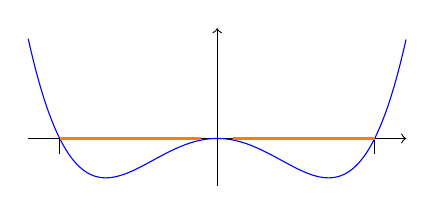
\begin{tikzpicture}[scale=2]
  \draw[->] (-1.2,0) -- (1.2,0);
  \draw[->] (0,-.3) -- (0,.7);
  \foreach \x in {-1 ,..., 1} \draw (\x,-0.1) -- (\x,0);
  \draw [blue,domain=-1.2:1.2,samples=200,variable=\x] plot(\x,{\x*\x*\x*\x - \x*\x});
  \draw[very thick,orange] ( -1,0) -- (-0.1,0);
  \draw[very thick,orange] (0.1,0) -- (1,0);
 \end{tikzpicture}
\end{center}

\begin{center}
 \begin{tikzpicture}[scale=0.5]
  \draw[->] (-5,0) -- (5,0);
  \draw[->] (0,-5) -- (0,5);
  \foreach \x in {-5 ,..., 5} \draw (\x,-0.1) -- (\x,0);
  \foreach \y in {-5 ,..., 5} \draw (-0.1,\y) -- (0,\y);
  \draw[red] (-5,-5) -- (-4,-5);
  \draw[dotted] (-4,-5) -- (-4,-4);
  \draw[red] (-4,-4) -- (-3,-4);
  \draw[dotted] (-3,-4) -- (-3,-3);
  \draw[red] (-3,-3) -- (-2,-3);
  \draw[dotted] (-2,-3) -- (-2,-2);
  \draw[red] (-2,-2) -- (-1,-2);
  \draw[dotted] (-1,-2) -- (-1,-1);
  \draw[red] (-1,-1) -- ( 0,-1);
  \draw[dotted] ( 0,-1) -- ( 0, 0);
  \draw[red] ( 0, 0) -- ( 1, 0);
  \draw[dotted] ( 1, 0) -- ( 1, 1);
  \draw[red] ( 1, 1) -- ( 2, 1);
  \draw[dotted] ( 2, 1) -- ( 2, 2);
  \draw[red] ( 2, 2) -- ( 3, 2);
  \draw[dotted] ( 3, 2) -- ( 3, 3);
  \draw[red] ( 3, 3) -- ( 4, 3);
  \draw[dotted] ( 4, 3) -- ( 4, 4);
  \draw[red] ( 4, 4) -- ( 5, 4);
  \fill (-5,-5) circle(0.05);
  \fill (-4,-4) circle(0.05);
  \fill (-3,-3) circle(0.05);
  \fill (-2,-2) circle(0.05);
  \fill (-1,-1) circle(0.05);
  \fill (0,0) circle(0.05);
  \fill (1,1) circle(0.05);
  \fill (2,2) circle(0.05);
  \fill (3,3) circle(0.05);
  \fill (4,4) circle(0.05);
 \end{tikzpicture}
\end{center}

\begin{center}
 \begin{tikzpicture}[scale=0.6]
  \draw[->] (-5,0) -- (5,0);
  \draw[->] (0,-1.5) -- (0,1.5);
  \foreach \x in {-5 ,..., 5} \draw (\x,-0.1) -- (\x,0);
  \foreach \y in {-1 ,..., 1} \draw (-0.1,\y) -- (0,\y);
  \draw[red] (-5,-1) -- (-4,-1);
  \draw[dotted] (-4,-1) -- (-4,+1);
  \draw[red] (-4,+1) -- (-3,+1);
  \draw[dotted] (-3,+1) -- (-3,-1);
  \draw[red] (-3,-1) -- (-2,-1);
  \draw[dotted] (-2,-1) -- (-2,+1);
  \draw[red] (-2,+1) -- (-1,+1);
  \draw[dotted] (-1,+1) -- (-1,-1);
  \draw[red] (-1,-1) -- ( 0,-1);
  \draw[dotted] ( 0,-1) -- ( 0,+1);
  \draw[red] ( 0,+1) -- ( 1,+1);
  \draw[dotted] ( 1,+1) -- ( 1,-1);
  \draw[red] ( 1,-1) -- ( 2,-1);
  \draw[dotted] ( 2,-1) -- ( 2,+1);
  \draw[red] ( 2,+1) -- ( 3,+1);
  \draw[dotted] ( 3,+1) -- ( 3,-1);
  \draw[red] ( 3,-1) -- ( 4,-1);
  \draw[dotted] ( 4,-1) -- ( 4,+1);
  \draw[red] ( 4,+1) -- ( 5,+1);
  \fill (-5,-1) circle(0.05);
  \fill (-4,+1) circle(0.05);
  \fill (-3,-1) circle(0.05);
  \fill (-2,+1) circle(0.05);
  \fill (-1,-1) circle(0.05);
  \fill (0,+1) circle(0.05);
  \fill (1,-1) circle(0.05);
  \fill (2,+1) circle(0.05);
  \fill (3,-1) circle(0.05);
  \fill (4,+1) circle(0.05);
 \end{tikzpicture}
\end{center}

\begin{center}
 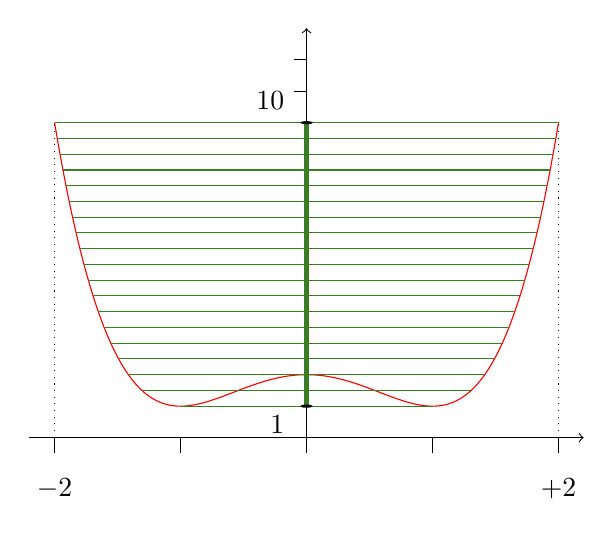
\begin{tikzpicture}[xscale=1.6,yscale=0.4]
  \def\ff(#1){{(#1*#1*#1*#1-2*#1*#1+2)}}
  \def\gg(#1){sqrt(sqrt(#1 - 1)+1)}
  \draw[->] (-2.2,0) -- (2.2,0);
  \draw[->] (0,0) -- (0,13);
  \foreach \x in {-2,-1,0,1,2} \draw (\x,-0.5) -- (\x,0);
  \foreach \y in {0 ,..., 12} \draw (-0.1,\y) -- (0,\y);
  \draw[dotted] (-2,0) -- (-2,10);
  \draw[dotted] (+2,0) -- (+2,10);
  \draw [red,domain=-2:2,samples=200,variable=\x] plot(\x,{\ff(\x)});
  \foreach \y in {1.0,1.5,...,10} {
   \draw[olivegreen] ({-\gg(\y)},\y) -- ({\gg(\y)},\y);
  }
  \draw[ultra thick,olivegreen] (0,1) -- (0,10);
  \draw (-2,-1) node[anchor=north] {$-2$};
  \draw (+2,-1) node[anchor=north] {$+2$};
  \fill (0,1) circle(0.05);
  \fill (0,10) circle(0.05);
  \draw (-0.1,1.0) node[anchor=north east] {$1$};
  \draw (-0.1,10.1) node[anchor=south east] {$10$};
 \end{tikzpicture}
\end{center}

\begin{center}
 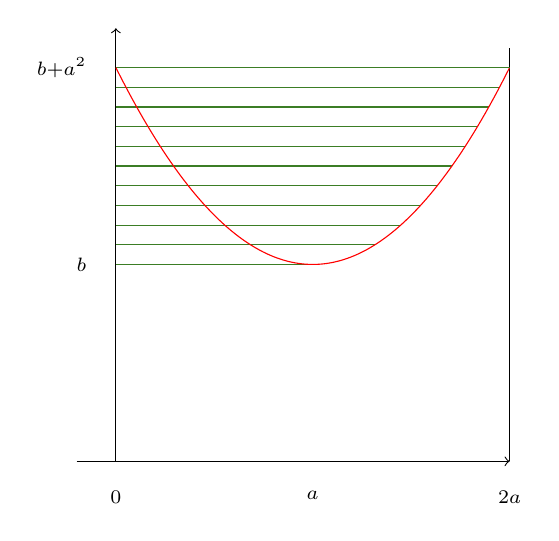
\begin{tikzpicture}[scale=2.5]
  \draw[->] (-0.2,0) -- (2,0);
  \draw[->] (0,0) -- (0,2.2);
  \draw (2,0) -- (2,2.1);
  \begin{scope}[draw=olivegreen]
   \draw ( 1,      1.0) -- (0,1.0);
   \draw ( 1.31623,1.1) -- (0,1.1);
   \draw ( 1.44721,1.2) -- (0,1.2);
   \draw ( 1.54772,1.3) -- (0,1.3);
   \draw ( 1.63246,1.4) -- (0,1.4);
   \draw ( 1.70711,1.5) -- (0,1.5);
   \draw ( 1.7746 ,1.6) -- (0,1.6);
   \draw ( 1.83666,1.7) -- (0,1.7);
   \draw ( 1.89443,1.8) -- (0,1.8);
   \draw ( 1.94868,1.9) -- (0,1.9);
   \draw ( 2.     ,2.0) -- (0,2.0);
  \end{scope}
  \draw[red,domain=0:2,samples=100,variable=\x] plot(\x,{(\x-1)*(\x-1)+1});
  \draw (0,-0.1) node[anchor=north] {$\scriptstyle 0$};
  \draw (1,-0.1) node[anchor=north] {$\scriptstyle a$};
  \draw (2,-0.1) node[anchor=north] {$\scriptstyle 2a$};
  \draw (-0.1,1) node[anchor=east] {$\scriptstyle b$};
  \draw (-0.1,2) node[anchor=east] {$\scriptstyle b+a^2$};
 \end{tikzpicture}
\end{center}

\begin{center}
 \begin{tikzpicture}[xscale=0.7,yscale=3]
  \draw[->] (0,0) -- (13,0);
  \draw[->] (0,-1.2) -- (0,1.2);
  \draw[yellow,domain=0:1,samples=20,variable=\x] plot(\x,{sin(30*\x)});
  \draw[red   ,domain=1:7,samples=120,variable=\x] plot(\x,{sin(30*\x)});
  \draw[yellow,domain=7:12,samples=100,variable=\x] plot(\x,{sin(30*\x)});
  \begin{scope}[draw=olivegreen]
   \draw (7., -0.5) -- (0,-0.5);
   \draw (6.78594, -0.4) -- (0,-0.4);
   \draw (6.58192, -0.3) -- (0,-0.3);
   \draw (6.38457, -0.2) -- (0,-0.2);
   \draw (6.19131, -0.1) -- (0,-0.1);
   \draw (6., 0.) -- (0,0.);
   \draw (5.80869, 0.1) -- (0,0.1);
   \draw (5.61543, 0.2) -- (0,0.2);
   \draw (5.41808, 0.3) -- (0,0.3);
   \draw (5.21406, 0.4) -- (0,0.4);
   \draw (5., 0.5) -- (0,0.5);
   \draw (4.771, 0.6) -- (0,0.6);
   \draw (4.5191, 0.7) -- (0,0.7);
   \draw (4.229, 0.8) -- (0,0.8);
   \draw (3.8614,  0.9) -- (0, 0.9);
   \draw (3., 1.) -- (0,1.);
  \end{scope}
  \draw[blue] (1,0) -- (1,.5);
  \draw[blue] (7,0) -- (7,-.5);
  \draw (-0.1,-0.5) node[anchor=east] {$\scriptstyle -1/2$};
  \draw (-0.1, 0.0) node[anchor=east] {$\scriptstyle 0$};
  \draw (-0.1, 0.5) node[anchor=east] {$\scriptstyle 1/2$};
  \draw (-0.1, 1.0) node[anchor=east] {$\scriptstyle 1$};
 \end{tikzpicture}
\end{center}

\begin{center}
 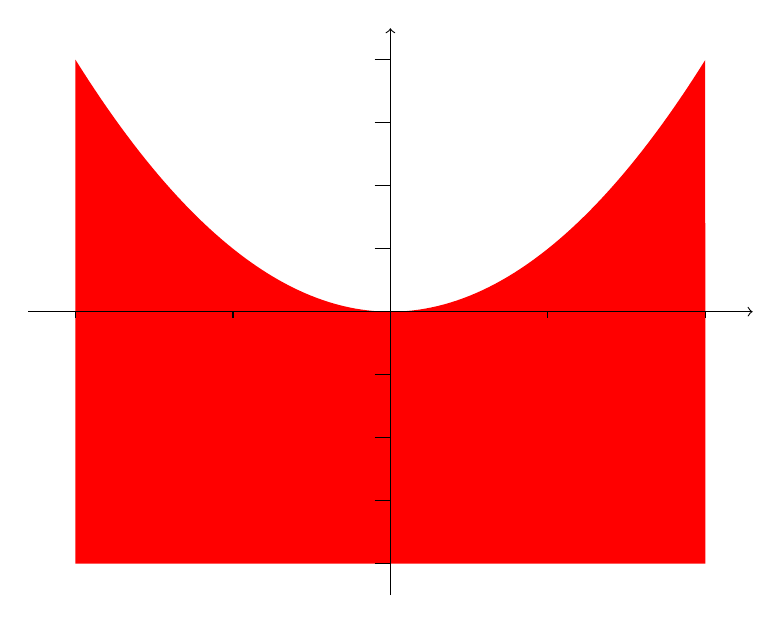
\begin{tikzpicture}[xscale=2,yscale=0.8]
  \fill[red   ,domain=-2:2,samples=100,variable=\x] plot(\x,{\x*\x}) -- (2,-4) -- (-2,-4) -- cycle;
  \draw[->] (-2.3,0) -- (2.3,0);
  \draw[->] (0,-4.5) -- (0,4.5);
  \foreach \x in {-2 ,..., 2} \draw (\x,-0.1) -- (\x,0);
  \foreach \y in {-4 ,..., 4} \draw (-0.1,\y) -- (0,\y);
 \end{tikzpicture}
\end{center}

\begin{center}
 \begin{tikzpicture}
  \draw (-4, 0) node {$A$};
  \draw (0, 0) node {$B$};
  \draw (4, 0) node {$C$} ;
  \draw (-4,-1) node {$a$};
  \draw (0,-1) node {$f(a)$};
  \draw (4,-1) node {$g(f(a))$} ;
  \draw[->] (-3.5, 0) -- (-0.5, 0);
  \draw[->] (+0.5, 0) -- (+3.5, 0);
  \draw (-2,.3) node {$f$};
  \draw (+2,.3) node {$g$};
  \draw[red,->] (-3.5,-1) -- (-0.7,-1); 
  \draw[red] (-3.5,-1.1) -- (-3.5,-0.9);
  \draw[red,->] (+0.7,-1) -- (+2.9,-1);
  \draw[red] (+0.7,-1.1) -- (+0.7,-0.9);
 \end{tikzpicture}
\end{center}

\begin{center}
 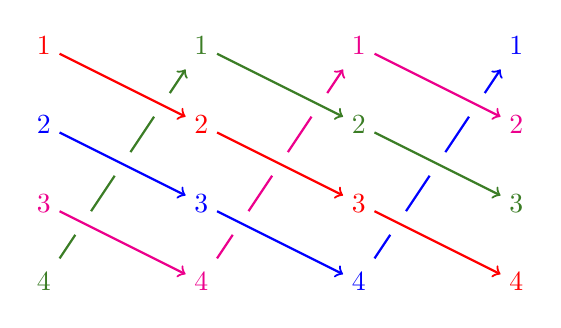
\begin{tikzpicture}[thick,xscale=2]
  \begin{scope}[draw=red,text=red]
   \draw (0,-1) node {$1$};
   \draw[->] (0.1,-1.1) -- (0.9,-1.9);
   \draw (1,-2) node {$2$};
   \draw[->] (1.1,-2.1) -- (1.9,-2.9);
   \draw (2,-3) node {$3$};
   \draw[->] (2.1,-3.1) -- (2.9,-3.9);
   \draw (3,-4) node {$4$};
  \end{scope}
  \begin{scope}[draw=blue,text=blue]
   \draw (0,-2) node {$2$};
   \draw[->] (0.1,-2.1) -- (0.9,-2.9);
   \draw (1,-3) node {$3$};
   \draw[->] (1.1,-3.1) -- (1.9,-3.9);
   \draw (2,-4) node {$4$};
   \draw (2.10,-3.70) -- (2.20,-3.40);
   \draw (2.30,-3.10) -- (2.45,-2.65);
   \draw (2.55,-2.35) -- (2.70,-1.90);
   \draw[->] (2.80,-1.60) -- (2.90,-1.30);
   \draw (3,-1) node {$1$};
  \end{scope}
  \begin{scope}[draw=magenta,text=magenta]
   \draw (0,-3) node {$3$};
   \draw[->] (0.1,-3.1) -- (0.9,-3.9);
   \draw (1,-4) node {$4$};
   \draw (1.10,-3.70) -- (1.20,-3.40);
   \draw (1.30,-3.10) -- (1.45,-2.65);
   \draw (1.55,-2.35) -- (1.70,-1.90);
   \draw[->] (1.80,-1.60) -- (1.90,-1.30);
   \draw (2,-1) node {$1$};
   \draw[->] (2.1,-1.1) -- (2.9,-1.9);
   \draw (3,-2) node {$2$};
  \end{scope}
  \begin{scope}[draw=olivegreen,text=olivegreen]
   \draw (0,-4) node {$4$};
   \draw (0.10,-3.70) -- (0.20,-3.40);
   \draw (0.30,-3.10) -- (0.45,-2.65);
   \draw (0.55,-2.35) -- (0.70,-1.90);
   \draw[->] (0.80,-1.60) -- (0.90,-1.30);
   \draw (1,-1) node {$1$};
   \draw[->] (1.1,-1.1) -- (1.9,-1.9);
   \draw (2,-2) node {$2$};
   \draw[->] (2.1,-2.1) -- (2.9,-2.9);
   \draw (3,-3) node {$3$};
  \end{scope}
 \end{tikzpicture}
\end{center}

\begin{center}
 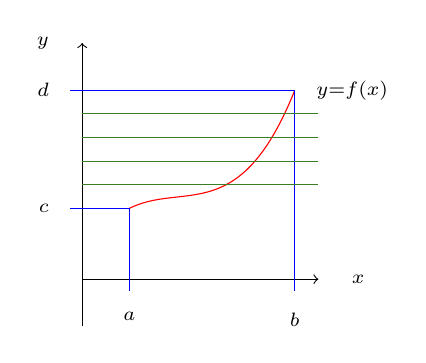
\begin{tikzpicture}[scale=3]
  \draw[->] (0,0) -- (1,0);
  \draw[->] (0,-0.2) -- (0,1);
  \draw[red,domain=0.2:0.9,samples=100,variable=\x] plot(\x,{3.175 *\x*\x*\x - 3.810 *\x*\x + 1.635*\x + 0.1});
  \draw[blue] (.2,-.05) -- (.2,.3) -- (-.05,.3);
  \draw[blue] (.9,-.05) -- (.9,.8) -- (-.05,.8);
  \draw[olivegreen] (0,.4) -- (1,.4);
  \draw[olivegreen] (0,.5) -- (1,.5);
  \draw[olivegreen] (0,.6) -- (1,.6);
  \draw[olivegreen] (0,.7) -- (1,.7);
  \draw (.2,-.1) node[anchor=north] {$\scriptstyle a$};
  \draw (.9,-.1) node[anchor=north] {$\scriptstyle b$};
  \draw (-.1,.3) node[anchor=east] {$\scriptstyle c$};
  \draw (-.1,.8) node[anchor=east] {$\scriptstyle d$};
  \draw (1.1,0) node[anchor=west] {$\scriptstyle x$};
  \draw (-0.1,1) node[anchor=east] {$\scriptstyle y$};
  \draw (0.95,0.8) node[anchor=west] {$\scriptstyle y=f(x)$};
 \end{tikzpicture}
\end{center}

\begin{center}
 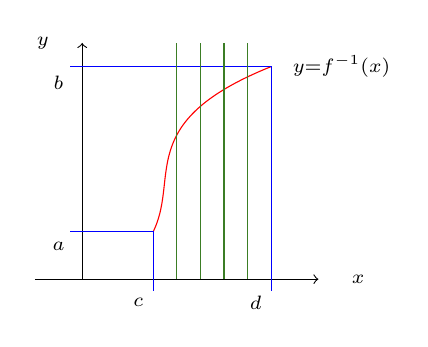
\begin{tikzpicture}[scale=3]
  \draw[->] (-0.2,0) -- (1,0);
  \draw[->] (0,0) -- (0,1);
  \draw[red,domain=0.2:0.9,samples=100,variable=\x] plot({3.175 *\x*\x*\x - 3.810 *\x*\x + 1.635*\x + 0.1},\x);
  \draw[blue] (-.05,.2) -- (.3,.2) -- (.3,-.05);
  \draw[blue] (-.05,.9) -- (.8,.9) -- (.8,-.05);
  \draw[olivegreen] (.4,0) -- (.4,1);
  \draw[olivegreen] (.5,0) -- (.5,1);
  \draw[olivegreen] (.6,0) -- (.6,1);
  \draw[olivegreen] (.7,0) -- (.7,1);
  \draw (-.1,.2) node[anchor=north] {$\scriptstyle a$};
  \draw (-.1,.9) node[anchor=north] {$\scriptstyle b$};
  \draw (.3,-.1) node[anchor=east] {$\scriptstyle c$};
  \draw (.8,-.1) node[anchor=east] {$\scriptstyle d$};
  \draw (1.1,0) node[anchor=west] {$\scriptstyle x$};
  \draw (-0.1,1) node[anchor=east] {$\scriptstyle y$};
  \draw (0.85,0.9) node[anchor=west] {$\scriptstyle y=f^{-1}(x)$};
 \end{tikzpicture}
\end{center}

\begin{center}
 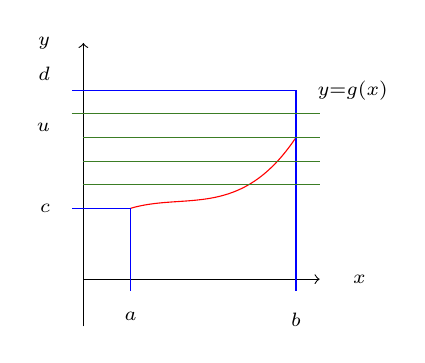
\begin{tikzpicture}[scale=3]
  \draw[->] (0,0) -- (1,0);
  \draw[->] (0,-0.2) -- (0,1);
  \draw[red,domain=0.2:0.9,samples=100,variable=\x] plot(\x,{1.905 *\x*\x*\x - 2.286*\x*\x + 0.981*\x + 0.180});
  \draw[blue] (.2,-.05) -- (.2,.3) -- (-.05,.3);
  \draw[blue] (.9,-.05) -- (.9,.8) -- (-.05,.8);
  \draw[olivegreen] (0,.4) -- (1,.4);
  \draw[olivegreen] (0,.5) -- (1,.5);
  \draw[olivegreen] (0,.6) -- (1,.6);
  \draw[olivegreen] (-.05,.7) -- (1,.7);
  \draw (.2,-.1) node[anchor=north] {$\scriptstyle a$};
  \draw (.9,-.1) node[anchor=north] {$\scriptstyle b$};
  \draw (-.1,.3) node[anchor=east] {$\scriptstyle c$};
  \draw (-.1,.8) node[anchor=south east] {$\scriptstyle d$};
  \draw (-.1,.7) node[anchor=north east] {$\scriptstyle u$};
  \draw (1.1,0) node[anchor=west] {$\scriptstyle x$};
  \draw (-0.1,1) node[anchor=east] {$\scriptstyle y$};
  \draw (0.95,0.8) node[anchor=west] {$\scriptstyle y=g(x)$};
 \end{tikzpicture}
\end{center}

\begin{center}
 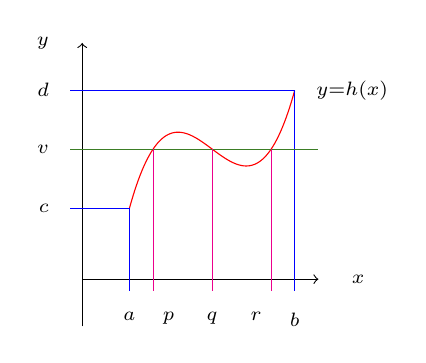
\begin{tikzpicture}[scale=3]
  \draw[->] (0,0) -- (1,0);
  \draw[->] (0,-0.2) -- (0,1);
  \draw[red,domain=0.2:0.9,samples=100,variable=\x] plot(\x,{11.905 *\x*\x*\x - 19.643*\x*\x + 10.060*\x -1.021});
  \draw[blue] (.2,-.05) -- (.2,.3) -- (-.05,.3);
  \draw[blue] (.9,-.05) -- (.9,.8) -- (-.05,.8);
  \draw[olivegreen] (-.05,.55) -- (1,.55);
  \draw[magenta] (0.30,-.05) -- (0.30,.55);
  \draw[magenta] (0.55,-.05) -- (0.55,.55);
  \draw[magenta] (0.80,-.05) -- (0.80,.55);
  \draw (.2,-.1) node[anchor=north] {$\scriptstyle a$};
  \draw (.3,-.1) node[anchor=north west] {$\scriptstyle p$};
  \draw (.55,-.1) node[anchor=north] {$\scriptstyle q$};
  \draw (.8,-.1) node[anchor=north east] {$\scriptstyle r$};
  \draw (.9,-.1) node[anchor=north] {$\scriptstyle b$};
  \draw (-.1,.3) node[anchor=east] {$\scriptstyle c$};
  \draw (-.1,.8) node[anchor=east] {$\scriptstyle d$};
  \draw (-.1,.55) node[anchor=east] {$\scriptstyle v$};
  \draw (1.1,0) node[anchor=west] {$\scriptstyle x$};
  \draw (-0.1,1) node[anchor=east] {$\scriptstyle y$};
  \draw (0.95,0.8) node[anchor=west] {$\scriptstyle y=h(x)$};
 \end{tikzpicture}
\end{center}

\begin{center}
 \begin{tikzpicture}[xscale=1.5,yscale=0.6]
  \draw[->] (-2.5,0) -- (2.5,0);
  \foreach \x in {-2 ,..., 2} \draw (\x,-0.1) -- (\x,0);
  \foreach \y in {0 ,..., 7} \draw (-0.1,\y) -- (0,\y);
  \draw[->] (0,0) -- (0,8);
  \draw[red,domain=-2:2.1,samples=100,variable=\x] plot(\x,{exp(\x)});
  \draw[olivegreen] (1,0) -- (1,2.72) -- (0,2.72);
  \draw[olivegreen] (2,0) -- (2,7.39) -- (0,7.39);
  \fill (0,1) circle(0.05);
  \fill (0,2.72) circle(0.05);
  \fill (0,7.39) circle(0.05);
  \draw (-.2,1) node[anchor=east] {$1$};
  \draw (-.2,2.72) node[anchor=east] {$e$};
  \draw (-.2,7.39) node[anchor=east] {$e^2$};
  \draw (-2,-.3) node[anchor=north] {$-2$};
  \draw (-1,-.3) node[anchor=north] {$-1$};
  \draw ( 0,-.3) node[anchor=north] {$0$};
  \draw ( 1,-.3) node[anchor=north] {$1$};
  \draw ( 2,-.3) node[anchor=north] {$2$};
  \draw (2.1,7.39) node[anchor=west] {$y=\exp(x)$};
 \end{tikzpicture}
\end{center}

\begin{center}
 \begin{tikzpicture}[xscale=0.8]
  \draw[->] (0,-2.5) -- (0,2.5);
  \foreach \x in {0 ,..., 7} \draw (\x,-0.1) -- (\x,0);
  \foreach \y in {-2 ,..., 2} \draw (-0.1,\y) -- (0,\y);
  \draw[->] (0,0) -- (8,0);
  \draw[red,domain=-2:2.1,samples=100,variable=\x] plot({exp(\x)},\x);
  \draw[olivegreen] (0,1) -- (2.72,1) -- (2.72,0);
  \draw[olivegreen] (0,2) -- (7.39,2) -- (7.39,0);
  \fill (1,0) circle(0.05);
  \fill (2.72,0) circle(0.05);
  \fill (7.39,0) circle(0.05);
  \draw (1,-.2) node[anchor=north] {$1$};
  \draw (2.72,-.2) node[anchor=north] {$e$};
  \draw (7.39,-.2) node[anchor=north] {$e^2$};
  \draw (-.3,-2) node[anchor=east] {$-2$};
  \draw (-.3,-1) node[anchor=east] {$-1$};
  \draw (-.3, 0) node[anchor=east] {$0$};
  \draw (-.3, 1) node[anchor=east] {$1$};
  \draw (-.3, 2) node[anchor=east] {$2$};
  \draw (3.2,1) node[anchor=west] {$y=\log(x)$};
  \draw (8.3,0) node[anchor=west] {$x$};
  \draw (0.3,2.5) node[anchor=west] {$y$};
 \end{tikzpicture}
\end{center}

\begin{center}
 \begin{tikzpicture}[xscale=2,yscale=1]
  \draw[red,domain=-2:2,samples=100,variable=\x] plot(\x,{(exp(\x)-exp(-\x))/2});
  \draw[olivegreen,domain=-2:2,samples=100,variable=\x] plot(\x,{(exp(\x)+exp(-\x))/2});
  \draw[blue,domain=-2:2,samples=100,variable=\x] plot(\x,{(exp(\x)-exp(-\x))/(exp(\x)+exp(-\x))});
  \draw[->] (-2.3,0) -- (2.5,0);
  \draw[->] (0,-4.3) -- (0,4.5);
  \foreach \x in {-2 ,..., 2} \draw (\x,-0.1) -- (\x,0);
  \foreach \y in {-4 ,..., 4} \draw (-0.1,\y) -- (0,\y);
  \draw[dotted] (-2.3,-1) -- (2.3,-1);
  \draw[dotted] (-2.3,+1) -- (2.3,+1);
  \draw (1.7,1.77) node {$\sinh(x)$};
  \draw (0.4,1.43) node {$\cosh(x)$};
  \draw (1.5,0.61) node {$\tanh(x)$};
  \draw (-0.1,+1.1) node[anchor=south east] {$1$};
  \draw (+0.1,-1.1) node[anchor=north west] {$-1$};
 \end{tikzpicture}
\end{center}

\begin{center}
 \begin{tikzpicture}[scale=4]
  \draw[->] (-1.2,0) -- (1.2,0);
  \draw[->] (0,-0.3) -- (0,1.2);
  \foreach \x in {-1 ,..., 1} \draw (\x,-0.1) -- (\x,0);
  \foreach \y in {0 ,..., 1} \draw (-0.1,\y) -- (0,\y);
  \fill(1,0) circle(0.015);
  \fill(0.5,0.87) circle(0.015);
  \draw[red] (0,0) (1,0) arc(0:180:1);
  \draw[red] (0,0) (0.2,0) arc(0:60:0.2);
  \draw[blue] (0,0) -- (0.5,0.87);
  \draw[magenta] (-.3,0.87) -- (0.5,0.87) -- (0.5,-.3);
  \draw[->] (-.15,0) -- (-.15,0.87);
  \draw[->] (-.15,0.87) -- (-.15,0);
  \draw[->] (0,-.15) -- (0.5,-.15);
  \draw[->] (0.5,-.15) -- (0,-.15);
  \draw (.25,-.2) node[anchor=north] {$\cos(\theta)$};
  \draw (-.2,.43) node[anchor=east] {$\sin(\theta)$};
  \draw (.55,.91) node[anchor=south west] {$P=(\cos(\theta),\sin(\theta))$};
  \draw (1.05,-.05) node[anchor=north west] {$A=(1,0)$};
  \draw (.26,.15) node {$\theta$};
 \end{tikzpicture}
\end{center}

\begin{center}
 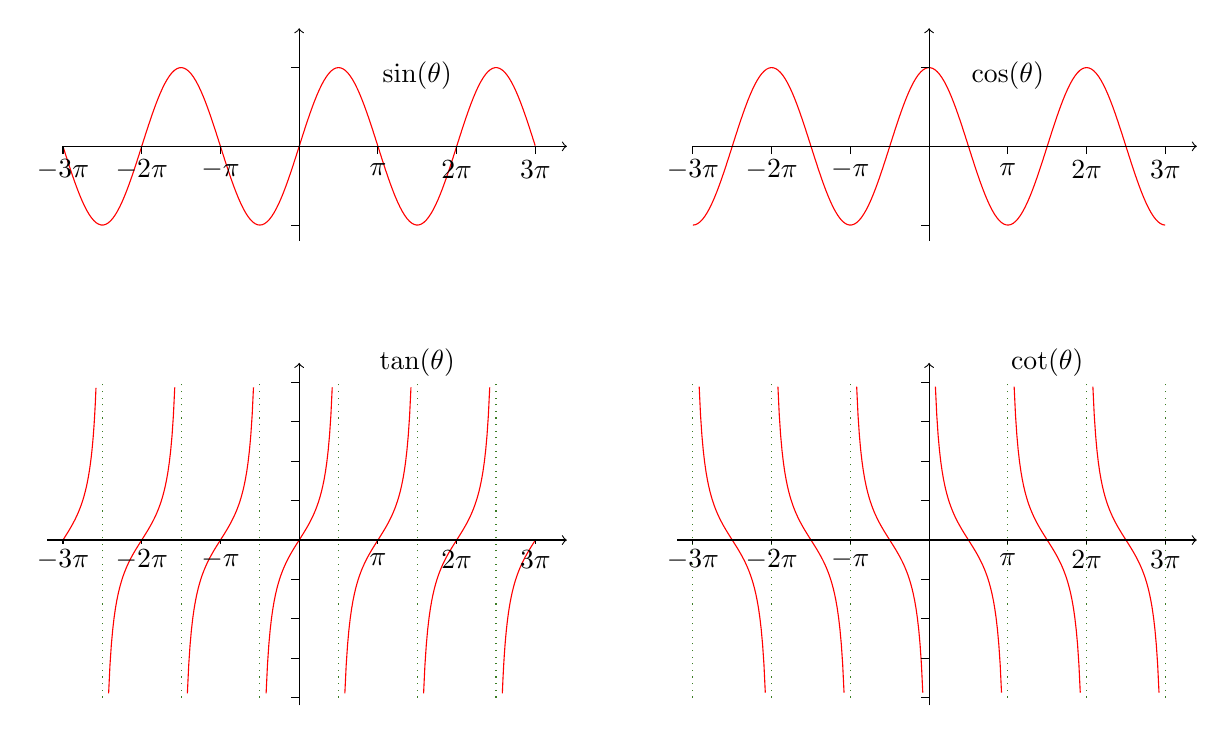
\begin{tikzpicture}
  \begin{scope}
   \draw[red,domain=-3:3,samples=200,variable=\x] plot(\x,{sin(180*\x)});
   \draw (-3,-.3) node {$-3\pi$};
   \draw (-2,-.3) node {$-2\pi$};
   \draw (-1,-.3) node {$-\pi$} ;
   \draw ( 1,-.3) node {$\pi$};
   \draw ( 2,-.3) node {$2\pi$};
   \draw ( 3,-.3) node {$3\pi$} ;
   \draw ( 1.5, .9) node {$\sin(\theta)$};
   \draw[->] (-3,0) -- (3.4,0);
   \draw[->] (0,-1.2) -- (0,1.5);
   \foreach \x in {-3 ,..., 3} \draw (\x,-0.1) -- (\x,0);
   \foreach \y in {-1 ,..., 1} \draw (-0.1,\y) -- (0,\y);
  \end{scope}
  \begin{scope}[shift={(8,0)}]
   \draw[red,domain=-3:3,samples=200,variable=\x] plot(\x,{cos(180*\x)});
   \draw (-3,-.3) node {$-3\pi$};
   \draw (-2,-.3) node {$-2\pi$};
   \draw (-1,-.3) node {$-\pi$} ;
   \draw ( 1,-.3) node {$\pi$};
   \draw ( 2,-.3) node {$2\pi$};
   \draw ( 3,-.3) node {$3\pi$} ;
   \draw ( 1, .9) node {$\cos(\theta)$};
   \draw[->] (-3,0) -- (3.4,0);
   \draw[->] (0,-1.2) -- (0,1.5);
   \foreach \x in {-3 ,..., 3} \draw (\x,-0.1) -- (\x,0);
   \foreach \y in {-1 ,..., 1} \draw (-0.1,\y) -- (0,\y);
  \end{scope}
  \begin{scope}[yshift=-5cm,yscale=0.5]
   \draw[red,domain=-3.00:-2.58,samples=50,variable=\x] plot(\x,{tan(180*\x)});
   \draw[red,domain=-2.42:-1.58,samples=50,variable=\x] plot(\x,{tan(180*\x)});
   \draw[red,domain=-1.42:-0.58,samples=50,variable=\x] plot(\x,{tan(180*\x)});
   \draw[red,domain=-0.42: 0.42,samples=50,variable=\x] plot(\x,{tan(180*\x)});
   \draw[red,domain= 0.58: 1.42,samples=50,variable=\x] plot(\x,{tan(180*\x)});
   \draw[red,domain= 1.58: 2.42,samples=50,variable=\x] plot(\x,{tan(180*\x)});
   \draw[red,domain= 2.58: 3.00,samples=50,variable=\x] plot(\x,{tan(180*\x)});
   \draw[dotted,olivegreen] (-2.5,-4) -- (-2.5,4);
   \draw[dotted,olivegreen] (-1.5,-4) -- (-1.5,4);
   \draw[dotted,olivegreen] (-0.5,-4) -- (-0.5,4);
   \draw[dotted,olivegreen] ( 0.5,-4) -- ( 0.5,4);
   \draw[dotted,olivegreen] ( 1.5,-4) -- ( 1.5,4);
   \draw[dotted,olivegreen] ( 2.5,-4) -- ( 2.5,4);
   \draw (-3,-.5) node {$-3\pi$};
   \draw (-2,-.5) node {$-2\pi$};
   \draw (-1,-.5) node {$-\pi$} ;
   \draw ( 1,-.5) node {$\pi$};
   \draw ( 2,-.5) node {$2\pi$};
   \draw ( 3,-.5) node {$3\pi$} ;
   \draw ( 1.5, 4.5) node {$\tan(\theta)$};
   \draw[->] (-3.2,0) -- (3.4,0);
   \draw[->] (0,-4.2) -- (0,4.5);
   \foreach \x in {-3 ,..., 3} \draw (\x,-0.1) -- (\x,0);
   \foreach \y in {-4 ,..., 4} \draw (-0.1,\y) -- (0,\y);
  \end{scope}
  \begin{scope}[xshift=8cm,yshift=-5cm,yscale=0.5]
   \draw[red,domain=-2.92:-2.08,samples=50,variable=\x] plot(\x,{1/tan(180*\x)});
   \draw[red,domain=-1.92:-1.08,samples=50,variable=\x] plot(\x,{1/tan(180*\x)});
   \draw[red,domain=-0.92:-0.08,samples=50,variable=\x] plot(\x,{1/tan(180*\x)});
   \draw[red,domain= 0.08: 0.92,samples=50,variable=\x] plot(\x,{1/tan(180*\x)});
   \draw[red,domain= 1.08: 1.92,samples=50,variable=\x] plot(\x,{1/tan(180*\x)});
   \draw[red,domain= 2.08: 2.92,samples=50,variable=\x] plot(\x,{1/tan(180*\x)});
   \draw[dotted,olivegreen] (-3,-4) -- (-3,4);
   \draw[dotted,olivegreen] (-2,-4) -- (-2,4);
   \draw[dotted,olivegreen] (-1,-4) -- (-1,4);
   \draw[dotted,olivegreen] ( 0,-4) -- ( 0,4);
   \draw[dotted,olivegreen] ( 1,-4) -- ( 1,4);
   \draw[dotted,olivegreen] ( 2,-4) -- ( 2,4);
   \draw[dotted,olivegreen] ( 3,-4) -- ( 3,4);
   \draw (-3,-.5) node {$-3\pi$};
   \draw (-2,-.5) node {$-2\pi$};
   \draw (-1,-.5) node {$-\pi$} ;
   \draw ( 1,-.5) node {$\pi$};
   \draw ( 2,-.5) node {$2\pi$};
   \draw ( 3,-.5) node {$3\pi$} ;
   \draw ( 1.5, 4.5) node {$\cot(\theta)$};
   \draw[->] (-3.2,0) -- (3.4,0);
   \draw[->] (0,-4.2) -- (0,4.5);
   \foreach \x in {-3 ,..., 3} \draw (\x,-0.1) -- (\x,0);
   \foreach \y in {-4 ,..., 4} \draw (-0.1,\y) -- (0,\y);
  \end{scope}
 \end{tikzpicture}
\end{center}

\begin{center}
 \begin{tikzpicture}[scale=4]
 \begin{scope}
  \draw (0,0) -- (1,0) -- (0,1) -- (0,0);
  \draw[red] (.1,0) -- (.1,.1) -- (0,.1);
  \draw[red] (1,0) (0.8,0) arc(180:135:0.2);
  \draw[red] (0,1) (0,0.8) arc(270:315:0.2);
  \draw (.5,-.1) node[anchor=north] {$1$};
  \draw (-.1,.5) node[anchor=east] {$1$};
  \draw (.54,.54) node[anchor=south west] {$\sqrt{2}$};
  \draw (.10,.75) node {$\pi/4$};
  \draw (.70,.06) node {$\pi/4$};
  \draw (.11,.11) node[anchor=south west] {$\pi/2$};
 \end{scope}
 \begin{scope}[xshift=3cm,scale=1.2]
  \draw (0,0) -- (0,0.86) -- (0.5,0) -- (-0.5,0) -- (0,0.86);
  \draw[red] (-.1,0) -- (-.1,.1) -- (.1,.1) -- (.1,0);
  \draw[red] (-0.5,0) +(0:0.12) arc(0:60:0.12);
  \draw[red] ( 0.5,0) +(180:0.12) arc(180:120:0.12);
  \draw[red] (0,0.86) +(240:0.12) arc(240:300:0.12);
  \draw (-.4,.4) node[anchor=south east] {$1$};
  \draw ( .4,.4) node[anchor=south west] {$1$};
  \draw (-.25,-.07) node[anchor=north] {$1\over 2$};
  \draw ( .25,-.07) node[anchor=north] {$1\over 2$};
  \draw (-.07,.4) node[anchor=north] {$\sqrt{3}\over 2$};
  \draw (-.31,.12) node {$\pi\over 3$};
  \draw ( .31,.12) node {$\pi\over 3$};
  \draw (-.05,.65) node {$\pi\over 6$};
  \draw ( .05,.65) node {$\pi\over 6$};
 \end{scope}
 \end{tikzpicture}
\end{center}

\begin{center}
 \begin{tikzpicture}[scale=2]
 \begin{scope}
  \draw[->] (-1.2,0) -- (1.3,0);
  \draw[->] (0,-1.2) -- (0,1.3);
  \draw (-1,-.05) -- (-1,.05);
  \draw ( 1,-.05) -- ( 1,.05);
  \draw (-.05,-1) -- (.05,-1);
  \draw (-.05, 1) -- (.05, 1);
  \draw[red,domain=-1:1,samples=100,variable=\x] plot(\x,{sin(90*\x)});
  \draw (-1,-.1) node[anchor=north] {$-{\pi\over 2}$};
  \draw ( 1,-.1) node[anchor=north] {$\pi\over 2$};
  \draw (-.1, 1) node[anchor=east] {$1$};
  \draw (-.1,-1) node[anchor=east] {$-1$};
  \draw (.5,1) node {$\sin(x)$};
 \end{scope}
 \begin{scope}[shift={(3,0)}]
  \shift{(3,0)}
  \draw[->] (-1.2,0) -- (1.3,0);
  \draw[->] (0,-1.2) -- (0,1.3);
  \draw (-1,-.05) -- (-1,.05);
  \draw ( 1,-.05) -- ( 1,.05);
  \draw (-.05,-1) -- (.05,-1);
  \draw (-.05, 1) -- (.05, 1);
  \draw[red,domain=-1:1,samples=100,variable=\x] plot({sin(90*\x)},\x);
  \draw (-.1,-1) node[anchor=east] {$-{\pi\over 2}$};
  \draw (-.1, 1) node[anchor=east] {$\pi\over 2$};
  \draw (-1,-.1) node[anchor=north] {$-1$};
  \draw ( 1,-.1) node[anchor=north] {$1$};
  \draw (.5,1) node {$\arcsin(x)$};
 \end{scope}
 \end{tikzpicture}
\end{center}


\begin{center}
 \begin{tikzpicture}[scale=2]
 \begin{scope}
  \draw[->] (-.2,0) -- (2.3,0);
  \draw[->] (0,-1.2) -- (0,1.3);
  \draw ( 2,-.05) -- ( 2,.05);
  \draw (-.05,-1) -- (.05,-1);
  \draw (-.05, 1) -- (.05, 1);
  \draw[red,domain=0:2,samples=100,variable=\x] plot(\x,{cos(90*\x)});
  \draw ( 2,-.1) node[anchor=north] {$\pi$};
  \draw (-.1, 1) node[anchor=east] {$1$};
  \draw (-.1,-1) node[anchor=east] {$-1$};
  \draw (1,1) node {$\cos(x)$};
 \end{scope}
 \begin{scope}[shift={(4.5,-1)}]
  \draw[->] (-1.2,0) -- (1.3,0);
  \draw[->] (0,0) -- (0,2.3);
  \draw (-1,-.05) -- (-1,.05);
  \draw ( 1,-.05) -- ( 1,.05);
  \draw (-.05, 2) -- (.05, 2);
  \draw[red,domain=0:2,samples=100,variable=\x] plot({cos(90*\x)},\x);
  \draw (-.1, 2) node[anchor=east] {$\pi$};
  \draw (-1,-.1) node[anchor=north] {$-1$};
  \draw ( 0,-.1) node[anchor=north] {$0$};
  \draw ( 1,-.1) node[anchor=north] {$1$};
  \draw (.9,2) node {$\arccos(x)$};
 \end{scope}
 \end{tikzpicture}
\end{center}

\begin{center}
 \begin{tikzpicture}
  \begin{scope}
   \draw[->] (-1.2,0) -- (1.3,0);
   \draw[->] (0,-3.2) -- (0,3.3);
   \draw (-1,-.05) -- (-1,.05);
   \draw ( 1,-.05) -- ( 1,.05);
   \draw (-.05,-3) -- (.05,-3);
   \draw (-.05,-2) -- (.05,-2);
   \draw (-.05,-1) -- (.05,-1);
   \draw (-.05, 1) -- (.05, 1);
   \draw (-.05, 2) -- (.05, 2);
   \draw (-.05, 3) -- (.05, 3);
   \draw[red,domain=-0.8:0.8,samples=100,variable=\x] plot(\x,{tan(90*\x)});
   \draw[dotted,olivegreen] (-1,-3) -- (-1,3);
   \draw[dotted,olivegreen] ( 1,-3) -- ( 1,3);
   \draw (-1.05,-.1) node[anchor=north east] {$-{\pi\over 2}$};
   \draw ( 1.05,-.1) node[anchor=north west] {$\pi\over 2$};
   \draw (.9,3.3) node {$\tan(x)$};
  \end{scope}
  \begin{scope}[shift={(6,0)}]
   \shift{(6,0)}
   \draw[->] (-3.2,0) -- (3.3,0);
   \draw[->] (0,-1.2) -- (0,1.3);
   \draw (-.05,-1) -- (.05,-1);
   \draw (-.05, 1) -- (.05, 1);
   \draw (-3,-.05) -- (-3,.05);
   \draw (-2,-.05) -- (-2,.05);
   \draw (-1,-.05) -- (-1,.05);
   \draw ( 1,-.05) -- ( 1,.05);
   \draw ( 2,-.05) -- ( 2,.05);
   \draw ( 3,-.05) -- ( 3,.05);
   \draw[red,domain=-0.8:0.8,samples=100,variable=\x] plot({tan(90*\x)},\x);
   \draw[dotted,olivegreen] (-3,-1) -- (+3,-1);
   \draw[dotted,olivegreen] (-3,+1) -- (+3,+1);
   \draw (-.1,-1.05) node[anchor=north east] {$-{\pi\over 2}$};
   \draw (-.1, 1.05) node[anchor=south east] {$\pi\over 2$};
   \draw (1,1.5) node {$\arctan(x)$};
  \end{scope}
 \end{tikzpicture}
\end{center}

\begin{center}
 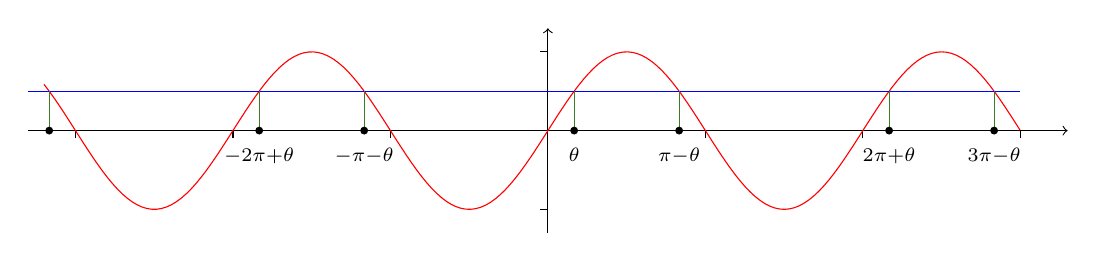
\begin{tikzpicture}
  \draw[->] (-6.6,0) -- (6.6,0);
  \draw[->] (0,-1.3) -- (0,1.3);
  \foreach \x in {-3 ,..., 3} \draw ({2*\x},-0.1) -- ({2*\x},0);
  \foreach \y in {-1 ,..., 1} \draw (-0.1,\y) -- (0,\y);
  \draw[red,domain=-3.2:3,samples=200,variable=\x] plot({2*\x},{sin(180*\x)});
  \draw[blue] (-6.6,.5) -- (6,.5);
  \begin{scope}[draw=olivegreen]
   \draw ({(-3-1/6)*2},.5) -- ({(-3-1/6)*2},0);
   \draw ({(-2+1/6)*2},.5) -- ({(-2+1/6)*2},0);
   \draw ({(-1-1/6)*2},.5) -- ({(-1-1/6)*2},0);
   \draw ({( 0+1/6)*2},.5) -- ({( 0+1/6)*2},0);
   \draw ({(+1-1/6)*2},.5) -- ({(+1-1/6)*2},0);
   \draw ({(+2+1/6)*2},.5) -- ({(+2+1/6)*2},0);
   \draw ({(+3-1/6)*2},.5) -- ({(+3-1/6)*2},0);
  \end{scope}
  \fill (-19/3,0) circle(0.05);
  \fill (-11/3,0) circle(0.05);
  \fill (- 7/3,0) circle(0.05);
  \fill (  1/3,0) circle(0.05);
  \fill (  5/3,0) circle(0.05);
  \fill ( 13/3,0) circle(0.05);
  \fill ( 17/3,0) circle(0.05);
  \draw (-11/3,-.1) node[anchor=north] {$\scriptstyle -2\pi+\theta$};
  \draw (- 7/3,-.1) node[anchor=north] {$\scriptstyle -\pi-\theta$};
  \draw (  1/3,-.1) node[anchor=north] {$\scriptstyle \theta$};
  \draw (  5/3,-.1) node[anchor=north] {$\scriptstyle \pi-\theta$};
  \draw ( 13/3,-.1) node[anchor=north] {$\scriptstyle 2\pi+\theta$};
  \draw ( 17/3,-.1) node[anchor=north] {$\scriptstyle 3\pi-\theta$};
 \end{tikzpicture}
\end{center}

\begin{center}
 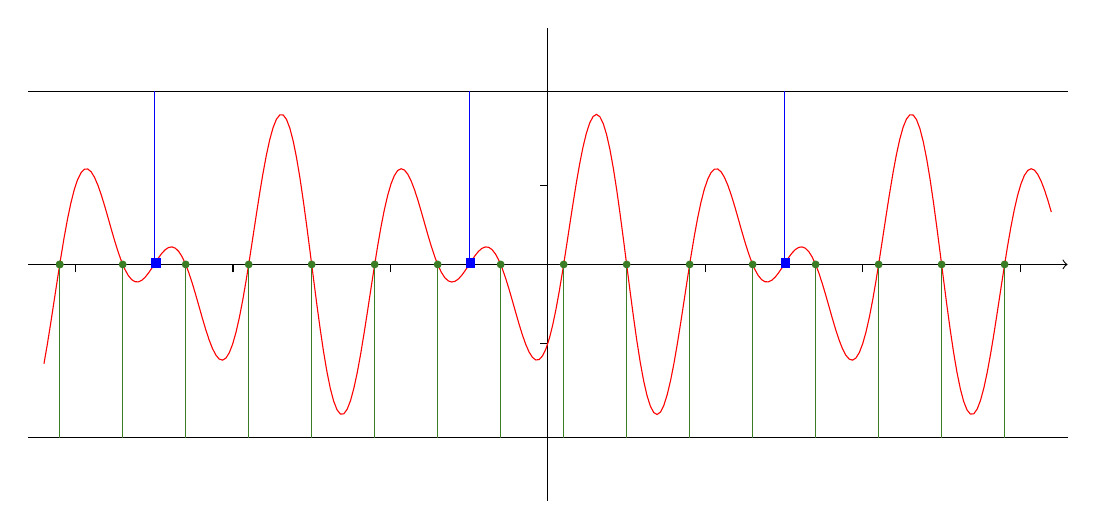
\begin{tikzpicture} % [50][30]{-3.3}{3.3}{-2.5}{2.5}
  \draw[->] (-6.6,0) -- (6.6,0);
  \foreach \x in {-3 ,..., 3} \draw ({2*\x},-0.1) -- ({2*\x},0);
  \foreach \y in {-1 ,..., 1} \draw (-0.1,\y) -- (0,\y);
  \draw (0,-3) -- (0,3);
  \draw (-6.6, 2.2) -- (6.6, 2.2);
  \draw (-6.6,-2.2) -- (6.6,-2.2);
  \draw[red,domain=-3.2:3.2,samples=300,variable=\x] plot({2*\x},{sin(360*\x)-cos(540*\x)});
  \fill[blue] (-5.0,0) +(-0.04,-0.04) rectangle +(0.08,0.08);
  \fill[blue] (-1.0,0) +(-0.04,-0.04) rectangle +(0.08,0.08);
  \fill[blue] ( 3.0,0) +(-0.04,-0.04) rectangle +(0.08,0.08);
  \draw[blue] (-5,0) -- (-5,2.2);
  \draw[blue] (-1,0) -- (-1,2.2);
  \draw[blue] ( 3,0) -- ( 3,2.2);
  \fill[olivegreen] ({-3.1 * 2},0) circle(0.05);
  \fill[olivegreen] ({-3.1 * 2},0) circle(0.05);
  \fill[olivegreen] ({-2.7 * 2},0) circle(0.05);
  \fill[olivegreen] ({-2.3 * 2},0) circle(0.05);
  \fill[olivegreen] ({-1.9 * 2},0) circle(0.05);
  \fill[olivegreen] ({-1.5 * 2},0) circle(0.05);
  \fill[olivegreen] ({-1.1 * 2},0) circle(0.05);
  \fill[olivegreen] ({-0.7 * 2},0) circle(0.05);
  \fill[olivegreen] ({-0.3 * 2},0) circle(0.05);
  \fill[olivegreen] ({ 0.1 * 2},0) circle(0.05);
  \fill[olivegreen] ({ 0.5 * 2},0) circle(0.05);
  \fill[olivegreen] ({ 0.9 * 2},0) circle(0.05);
  \fill[olivegreen] ({ 1.3 * 2},0) circle(0.05);
  \fill[olivegreen] ({ 1.7 * 2},0) circle(0.05);
  \fill[olivegreen] ({ 2.1 * 2},0) circle(0.05);
  \fill[olivegreen] ({ 2.5 * 2},0) circle(0.05);
  \fill[olivegreen] ({ 2.9 * 2},0) circle(0.05);
  \begin{scope}[draw=olivegreen]
   \draw ({-3.1 * 2},0) -- ({-3.1 * 2},-2.2);
   \draw ({-2.7 * 2},0) -- ({-2.7 * 2},-2.2);
   \draw ({-2.3 * 2},0) -- ({-2.3 * 2},-2.2);
   \draw ({-1.9 * 2},0) -- ({-1.9 * 2},-2.2);
   \draw ({-1.5 * 2},0) -- ({-1.5 * 2},-2.2);
   \draw ({-1.1 * 2},0) -- ({-1.1 * 2},-2.2);
   \draw ({-0.7 * 2},0) -- ({-0.7 * 2},-2.2);
   \draw ({-0.3 * 2},0) -- ({-0.3 * 2},-2.2);
   \draw ({ 0.1 * 2},0) -- ({ 0.1 * 2},-2.2);
   \draw ({ 0.5 * 2},0) -- ({ 0.5 * 2},-2.2);
   \draw ({ 0.9 * 2},0) -- ({ 0.9 * 2},-2.2);
   \draw ({ 1.3 * 2},0) -- ({ 1.3 * 2},-2.2);
   \draw ({ 1.7 * 2},0) -- ({ 1.7 * 2},-2.2);
   \draw ({ 2.1 * 2},0) -- ({ 2.1 * 2},-2.2);
   \draw ({ 2.5 * 2},0) -- ({ 2.5 * 2},-2.2);
   \draw ({ 2.9 * 2},0) -- ({ 2.9 * 2},-2.2);
  \end{scope}
 \end{tikzpicture}
\end{center}

\begin{center}
 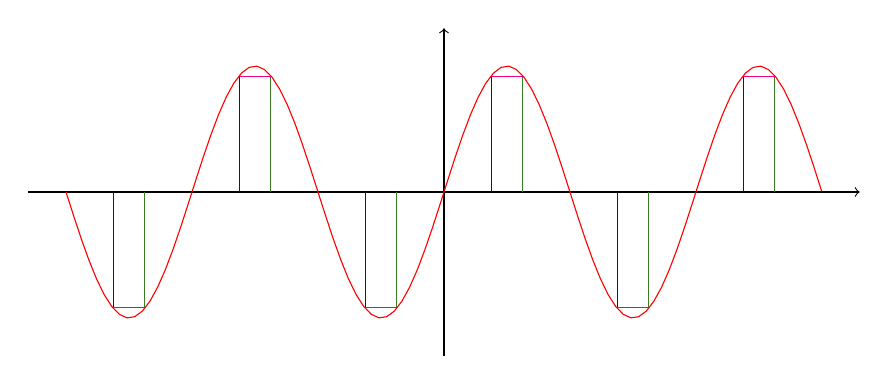
\begin{tikzpicture}[scale=1.6]
  \draw[->] (-3.3,0) -- (3.3,0);
  \draw[->] (0,-1.3) -- (0,1.3);
  \draw[red,domain=-3:3,samples=100,variable=\x] plot(\x,{sin(180*\x)});
  \begin{scope}[draw=blue]
   \draw (-3+3/8,0) -- (-3+3/8,-0.92);
   \draw (-2+3/8,0) -- (-2+3/8,+0.92);
   \draw (-1+3/8,0) -- (-1+3/8,-0.92);
   \draw ( 0+3/8,0) -- ( 0+3/8,+0.92);
   \draw ( 1+3/8,0) -- ( 1+3/8,-0.92);
   \draw ( 2+3/8,0) -- ( 2+3/8,+0.92);   
  \end{scope}
  \begin{scope}[draw=olivegreen]
   \draw (-3+5/8,0) -- (-3+5/8,-0.92);
   \draw (-2+5/8,0) -- (-2+5/8,+0.92);
   \draw (-1+5/8,0) -- (-1+5/8,-0.92);
   \draw ( 0+5/8,0) -- ( 0+5/8,+0.92);
   \draw ( 1+5/8,0) -- ( 1+5/8,-0.92);
   \draw ( 2+5/8,0) -- ( 2+5/8,+0.92);
  \end{scope}
  \begin{scope}[draw=magenta]
   \draw (-3+3/8,-0.92) -- (-3+5/8,-0.92);
   \draw (-2+3/8,+0.92) -- (-2+5/8,+0.92);
   \draw (-1+3/8,-0.92) -- (-1+5/8,-0.92);
   \draw ( 0+3/8,+0.92) -- ( 0+5/8,+0.92);
   \draw ( 1+3/8,-0.92) -- ( 1+5/8,-0.92);
   \draw ( 2+3/8,+0.92) -- ( 2+5/8,+0.92);
  \end{scope}
 \end{tikzpicture}
\end{center}

\begin{center}
 \begin{tikzpicture}[xscale=2]
  \draw[red,domain=-0.97:0.97,samples=100,variable=\x] plot(\x,{1/sqrt(1-\x*\x)});
  \draw[->] (-1.1,0) -- (1.2,0);
  \draw[->] (0,-0.5) -- (0,4.3);
  \foreach \x in {-1 ,..., 1} \draw (\x,-0.1) -- (\x,0);
  \foreach \y in {1 ,..., 4} \draw (-0.1,\y) -- (0,\y);
  \draw (-1,-0.1) node[anchor=north] {$-c$};
  \draw (+1,-0.1) node[anchor=north] {$+c$};
  \draw (1.3,0) node[anchor=west] {$v$};
  \draw (-0.05,0.95) node[anchor=north east] {$1$};
  \draw (-0.05,2) node[anchor=east] {$2$};
  \draw (-0.05,3) node[anchor=east] {$3$};
  \draw (-0.05,4) node[anchor=east] {$4$};
  \draw[blue,dotted] (-1,0) -- (-1,4);
  \draw[blue,dotted] (+1,0) -- (+1,4);
 \end{tikzpicture}
\end{center}

\begin{center}
 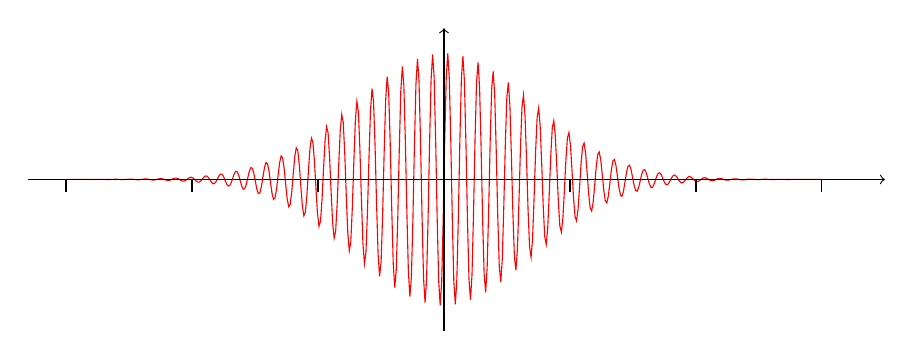
\begin{tikzpicture}[scale=1.6]
  \draw[red,domain=-3:3,samples=500,variable=\x] plot(\x,{exp(-\x*\x)*sin(3000*\x)});
  \draw[->] (-3.3,0) -- (3.5,0);
  \draw[->] (0,-1.2) -- (0,1.2);
  \foreach \x in {-3 ,..., 3} \draw (\x,-0.1) -- (\x,0);
 \end{tikzpicture}
\end{center}

\begin{center}
 \begin{tikzpicture}
  \draw[red,domain=-5:5,samples=600,variable=\x] plot(\x,{cos(200*\x*\x)});
  \drawcolor{black}
  \draw[->] [60](-5.5,0) -- (5.5,0);
  \draw[->] [60](0,-1.1) -- (0,1.1);
  \foreach \x in {-5 ,..., 5} \draw (\x,-0.1) -- (\x,0);
  \foreach \y in {-1,1} \draw (-0.1,\y) -- (0,\y);
 \end{tikzpicture}
\end{center}


\begin{center}
 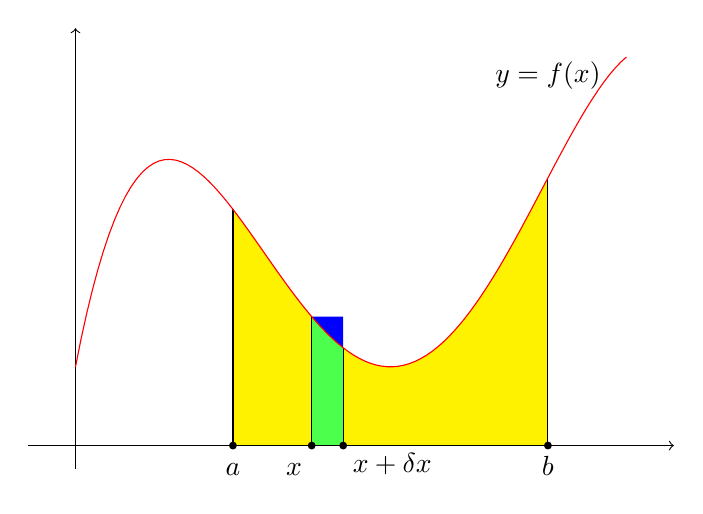
\begin{tikzpicture}
  \def\ff(#1){1+10.4*#1-12.8*#1*#1+5.0*#1*#1*#1-0.6*#1*#1*#1*#1}
  \fill[yellow,domain=1.0:3.0,samples=100,variable=\x]
    plot({2*\x},{\ff(\x)}) -- (6.0,0) -- (2.0,0) -- cycle;
  \fill[green!70,domain=1.5:1.7,samples=20,variable=\x]
    plot({2*\x},{\ff(\x)}) -- (3.4,0) -- (3.0,0) -- cycle;
  \fill[blue,domain=1.5:1.7,samples=20,variable=\x]
    plot({2*\x},{\ff(\x)}) -- (3.4,{\ff(1.5)}) -- cycle;
  \draw[->] (-0.6,0) -- (7.6,0);
  \draw[->] (0,-0.3) -- (0,5.3);
  \draw ({1.0 * 2},0) -- ({1.0 * 2},{\ff(1.0)});
  \draw ({1.5 * 2},0) -- ({1.5 * 2},{\ff(1.5)});
  \draw ({1.7 * 2},0) -- ({1.7 * 2},{\ff(1.7)});
  \draw ({3.0 * 2},0) -- ({3.0 * 2},{\ff(3.0)});
  \fill ({1.0 * 2},0) circle(0.05);
  \fill ({1.5 * 2},0) circle(0.05);
  \fill ({1.7 * 2},0) circle(0.05);
  \fill ({3.0 * 2},0) circle(0.05);
  \draw[red,domain=0:3.5,samples=100,variable=\x] plot({2*\x},{\ff(\x)});
  \draw ({1.0 * 2},-0.5) node[anchor=south] {$a$};
  \draw ({1.5 * 2},-0.5) node[anchor=south east] {$x$};
  \draw ({1.7 * 2},-0.5) node[anchor=south west] {$x+\delta{}x$};
  \draw ({3.0 * 2},-0.5) node[anchor=south] {$b$};
  \draw ({3.0 * 2},4.7) node {$y=f(x)$};
 \end{tikzpicture}
\end{center}

\begin{center}
 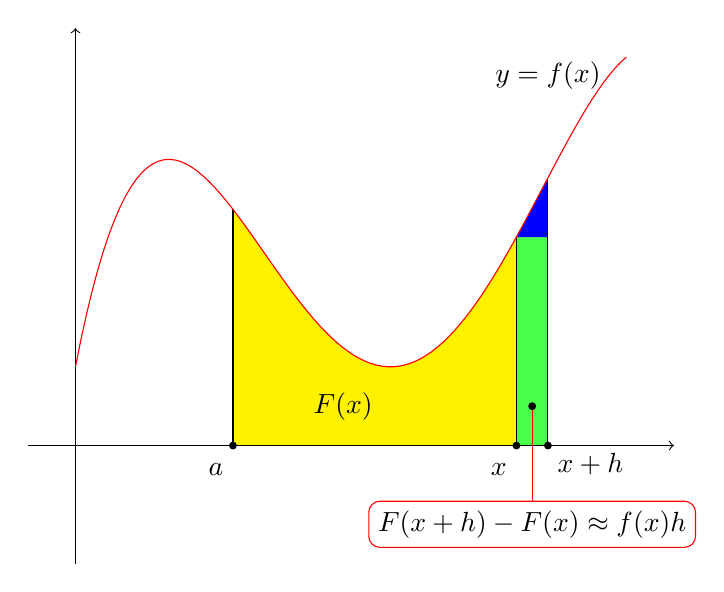
\begin{tikzpicture} % [60][30]{-0.3}{3.8}{-1.5}{5.3}
  \def\ff(#1){1+10.4*#1-12.8*#1*#1+5.0*#1*#1*#1-0.6*#1*#1*#1*#1}
  \fill[yellow,domain=1.0:2.8,samples=100,variable=\x]
    plot({2*\x},{\ff(\x)}) -- (5.6,0) -- (2.0,0) -- cycle;
  \fill[green!70,domain=2.8:3.0,samples=100,variable=\x]
    plot({2*\x},{\ff(\x)}) -- (6.0,0) -- (5.6,0) -- cycle;
  \fill[blue,domain=2.8:3.0,samples=100,variable=\x]
    plot({2*\x},{\ff(\x)}) -- (6.0,{\ff(2.8)}) -- cycle;
  \draw[->] (-0.6,0) -- (7.6,0);
  \draw[->] (0,-1.5) -- (0,5.3);
  \draw (2.0,0) -- (2.0,{\ff(1.0)});
  \draw (5.6,0) -- (5.6,{\ff(2.8)});
  \draw (6.0,0) -- (6.0,{\ff(3.0)});
  \fill (2.0,0) circle(0.05);
  \fill (5.6,0) circle(0.05);
  \fill (6.0,0) circle(0.05);
  \draw[red,domain=0:3.5,samples=100,variable=\x] plot({2*\x},{\ff(\x)});
  \draw (2.0,-0.5) node[anchor=south east] {$a$};
  \draw (5.6,-0.5) node[anchor=south east] {$x$};
  \draw (6.0,-0.5) node[anchor=south west] {$x+h$};
  \draw (3.4,0.5) node {$F(x)$};
  \draw (6.0,4.7) node {$y=f(x)$};
  \draw (5.8,-1.0) node[draw=red,text=black,rounded corners] {$F(x+h)-F(x)\approx f(x)h$};
  \draw[red] (5.8,-0.70) -- (5.8,0.5);
  \fill (5.8,0.5) circle(0.05);
 \end{tikzpicture}
\end{center}

\begin{center}
 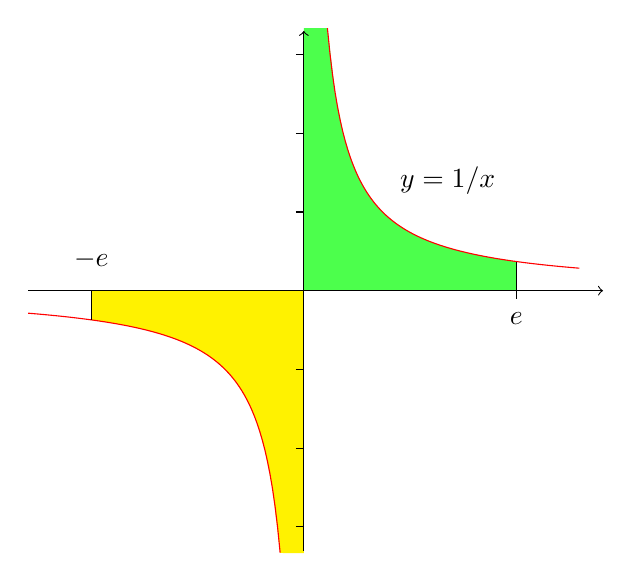
\begin{tikzpicture} % [25]{-3.5}{3.8}{-3.3}{3.3}
  \fill[yellow,domain=-2.7:-0.3,variable=\x]
    plot(\x,{1/\x}) -- (0,{-1/0.3}) -- (0,0) -- (-2.7,0) -- cycle;
  \fill[green!70,domain=0.3:2.7,variable=\x]
    plot(\x,{1/\x}) -- (2.7,0) -- (0,0) -- (0,{1/0.3}) -- cycle;
  \draw[red,domain=-3.5:-0.3,samples=100,variable=\x] plot(\x,{1/\x});
  \draw[red,domain=0.3:3.5  ,samples=100,variable=\x] plot(\x,{1/\x});
  \draw[->] (-3.5,0) -- (3.8,0);
  \draw[->] (0,-3.3) -- (0,3.3);
  \foreach \x in {-2.7,2.7} \draw (\x,-0.1) -- (\x,0);
  \foreach \y in {-3 ,..., 3} \draw (-0.1,\y) -- (0,\y);
  \draw (-2.7,0) -- (-2.7,-1/2.7);
  \draw (+2.7,0) -- (+2.7,+1/2.7);
  \draw (1.1,1.1) node[anchor=south west] {$y=1/x$};
  \draw (-2.7,+.15) node[anchor=south] {$-e$};
  \draw (+2.7,-.15) node[anchor=north] {$e$};
 \end{tikzpicture}
\end{center}

\begin{center}
 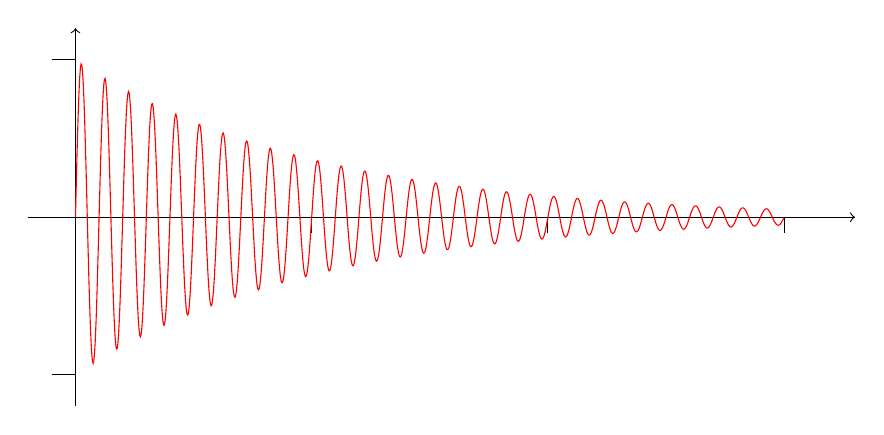
\begin{tikzpicture}[xscale=3,yscale=2]
  \draw[->] (-0.2,0) -- (3.3,0);
  \draw[->] (0,-1.2) -- (0,1.2);
  \foreach \x in {0,1,2,3} \draw (\x,-0.1) -- (\x,0);
  \foreach \y in {-1,1} \draw (-0.1,\y) -- (0,\y);
  \draw[red,domain=0:3,samples=1000,variable=\x] plot(\x,{sin(3600*\x)*exp(-\x)});
 \end{tikzpicture}
\end{center}


\end{document}
